\documentclass[11pt,english,table,dvipsnames]{beamer}
\usetheme{ubslides}

%\setbeameroption{show notes on second screen=right}

%%% set up literature
\setbeamertemplate{bibliography item}{\insertbiblabel}
\usepackage[%
  backend=bibtex      % biber or bibtex
%,style=authoryear    % Alphabeticalsch
 ,style=numeric-comp  % numerical-compressed
 ,sorting=none        % no sorting
 ,sortcites=true      % some other example options ...
 ,block=none
 ,indexing=false
 ,citereset=none
 ,isbn=true
 ,url=true
 ,doi=true            % prints doi
 ,natbib=true         % if you need natbib functions
]{biblatex}
\addbibresource{slides.bib}

% set up stuff for the title page and slides footer
\title[Bachelorthesis]{Design and Implementation of a high performance IPC for Intrusion Prevention using Socket API}
\subtitle{Bachelorthesis}
\author[Daniel von Rauchhaupt]{Daniel von Rauchhaupt}
\date{\today}
\institute[Uni Potsdam]{
\includegraphics[width=1.5cm]{./images/bsvs-logo}\\Universtität Potsdam\\ Institut für Informatik und Computational Science\\ Professur Betriebssysteme und Verteilte Systeme}

\lstset{
language=C,
breaklines=true,
breakatwhitespace=true,
frame=tb,
numbers=left,
stepnumber=1,
showstringspaces=false
}



\begin{document}

\begin{frame}[plain]
    \titlepage
\end{frame}

\begin{frame}
\frametitle{Agenda}
\tableofcontents[hidesubsections]
\end{frame}

\section{Motivation}
\begin{frame}{Motivation}
    Motivation
\end{frame}

\begin{frame}{Host-based intrusion detection and prevention}
    Threats\@:
    \begin{itemize}
        \item access data,
        \item manipulate data, or
        \item render a system unreliable or unusable.
    \end{itemize}
\end{frame}

\begin{frame}{Host-based intrusion detection and prevention}
    Necessity for Intrusion Prevention Systems\@:
    \begin{enumerate}
        \item The majority of systems have vulnerabilities, rendering them susceptible. 
        \item Replacing systems with known vulnerabilities is difficult. Specific features may only be present in the less-secure system.
        \item Developing absolutely secure systems is difficult, since the explicit absence of vulnerabilities can rarely be proven.
        \item Secure systems remain vulnerable to insiders misusing their privileges.
    \end{enumerate}
\end{frame}

\begin{frame}{Motivation - Fail2ban}
    Fail2ban application creates "jails"\@:
    \begin{enumerate}
        \item A jail consists out of\@:
            \begin{itemize}
                \item Log path
                \item Specific filter (uses Regex)
                \item A defined action
                \item Multiple customizable parameters (Ban duration, Ban limit)
            \end{itemize}
        \item Jails are saved on persistent storage
        \item Deduces vital client information from log messages
    \end{enumerate}
\end{frame}

\begin{frame}{Motivation - Fail2ban}
    \begin{center}
        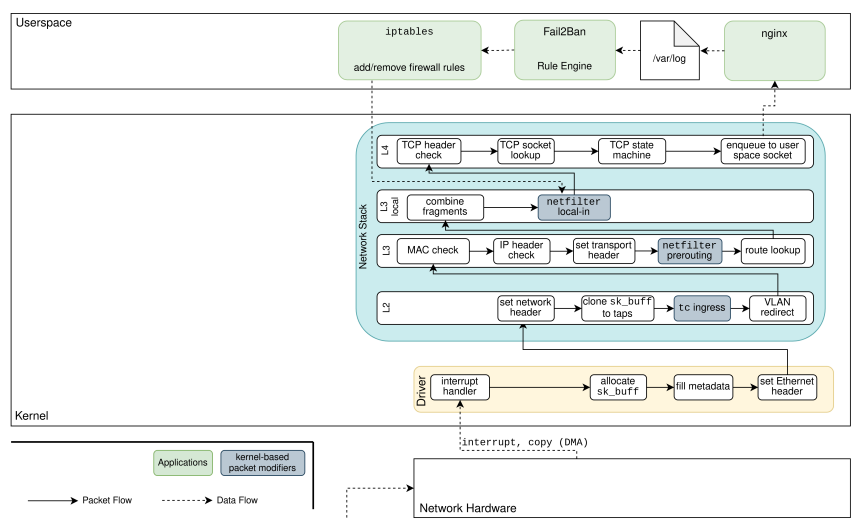
\includegraphics[width=0.8\linewidth]{images/Fail2ban_no_eBPF.PNG}
    \end{center}

    \let\thefootnote\relax\footnotetext{
        \tiny Florian Mikolajczak\@: Implementation and Evaluation\\ of an Intrusion Prevention System Leveraging eBPF on the Basis of Fail2Ban
    }
\end{frame}

\begin{frame}{Motivation - Fail2ban}
    \begin{center}
        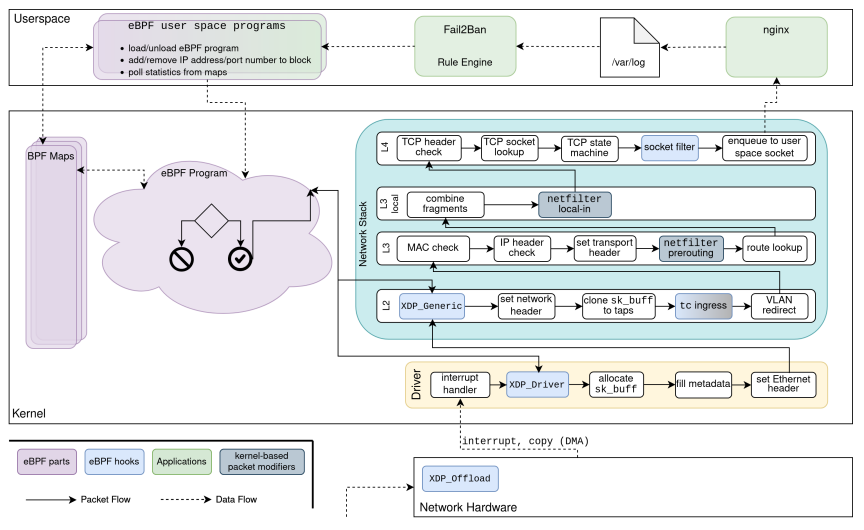
\includegraphics[width=0.8\linewidth]{images/Fail2ban_with_eBPF.PNG}
    \end{center}

    \let\thefootnote\relax\footnotetext{
        \tiny Florian Mikolajczak\@: Implementation and Evaluation\\ of an Intrusion Prevention System Leveraging eBPF on the Basis of Fail2Ban
    }
\end{frame}

\begin{frame}{Motivation - Fail2ban}
    \begin{center}
        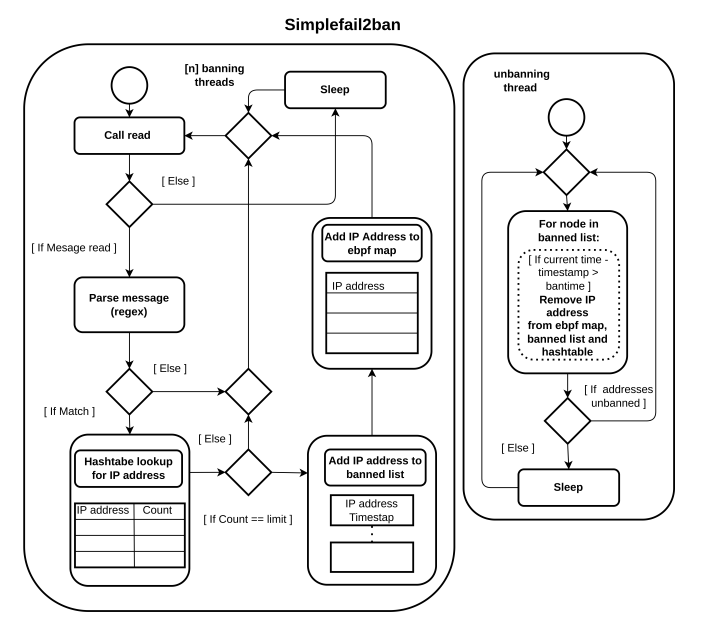
\includegraphics[width=0.6\linewidth]{images/Simplefail2ban_Design.PNG}
    \end{center}

    \let\thefootnote\relax\footnotetext{
        \tiny Paul Raatschen\@: Design and Implementation\\ of a new Inter-Process Communication Architecture for Log-based HIDS for 100 GbE Environments
    }
\end{frame}

\section{Design}
\begin{frame}{Design}
    Design
\end{frame}

\begin{frame}{UNIX domain sockets}
    An alternative to the shared memory mode\@: UNIX domain Sockets
    \\
    \begin{enumerate}
        \item Preferred over internet sockets
        \item Three types of UNIX domain sockets\@:
            \begin{itemize}
                \item SOCK\_STREAM\@: Stream-oriented socket. Establishes connections and keeps them open until explicitly closed.
                \item SOCK\_DGRAM\@: Datagram-oriented socket. Preserves message boundaries. Mostly reliable.
                \item SOCK\_SEQPACKET\@: Sequence-packet socket. Is connection-oriented, preserves message boundaries, and retains the order in which data was sent.
            \end{itemize}
    \end{enumerate}
\end{frame}

\begin{frame}{UNIX domain sockets}
    An alternative to the shared memory mode\@: UNIX domain Sockets
    \\
    \begin{enumerate}
        \item Preferred over internet sockets
        \item Three types of UNIX domain sockets\@:
            \begin{itemize}
                \item SOCK\_STREAM\@: Stream-oriented socket. Establishes connections and keeps them open until explicitly closed.
                \item SOCK\_DGRAM\@: Datagram-oriented socket. Preserves message boundaries. Mostly reliable.
                \item SOCK\_SEQPACKET\@: Sequence-packet socket. Is connection-oriented, preserves message boundaries, and retains the order in which data was sent.
            \end{itemize}
    \end{enumerate}
    \begin{block}{Block}
        -> SOCK\_SEQPACKET is preferred
    \end{block}
\end{frame}

\begin{frame}{UNIX domain sockets}
    An alternative to the shared memory mode\@:
    \begin{enumerate}
        \item Existing support on all UNIX systems
        \item Established Write and Read API
        \item Kernel-based IPC promising low latency and high bandwidth
        \item Easily scalable beyond the local system
    \end{enumerate}
\end{frame}

\begin{frame}{UNIX domain sockets}
    \begin{center}
        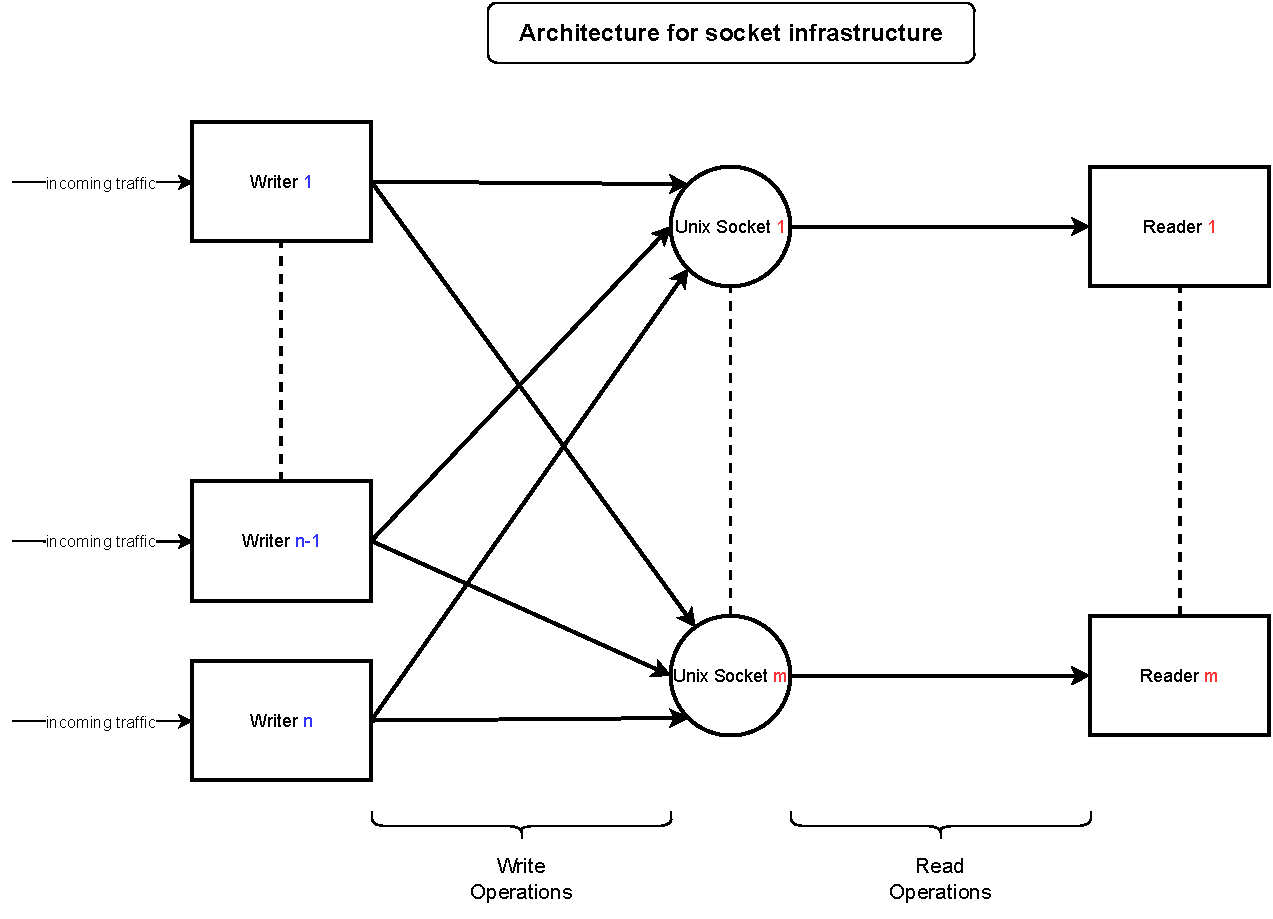
\includegraphics[width=0.8\linewidth]{images/SocketArchitecture.pdf}
    \end{center}
\end{frame}

\section{Implementation}
\begin{frame}{Implementation}
    Implementation
\end{frame}

\begin{frame}[fragile]{Shared parameters}
    \vfill
    Shared parameters\@:
    \vfill
    \begin{lstlisting}
#define MAX_AMOUNT_OF_SOCKETS 32
#define SOCKET_TEMPLATE_LENGTH 128
#define SOCKET_NAME_TEMPLATE "/tmp/unixDomainSock4SF2B_"
    \end{lstlisting}

    \vfill
    Union defining which process is calling a function\@:
    \vfill
    \begin{lstlisting}
union sock_arg_t{
    struct sock_writer_arg_t wargs;
    struct sock_reader_arg_t rargs;
};
    \end{lstlisting}
\end{frame}

\begin{frame}[fragile]{Auxiliary functions}
    \vfill
    Initialization of socket IPC\@:
    \vfill
    \begin{lstlisting}
int sock_init(
    union sock_arg_t *sock_args,
    int role
);
    \end{lstlisting}

    \vfill
    Cleanup of socket IPC\@:
    \vfill
    \begin{lstlisting}
int sock_cleanup(
    union sock_arg_t *sock_args,
    int role
);
    \end{lstlisting}
\end{frame}

\begin{frame}[fragile]{Write API}
    \vfill
    Writer structure\@:
    \vfill
    \begin{lstlisting}[breaklines]
struct sock_writer_arg_t
{
    char socketPathNames [MAX_AMOUNT_OF_SOCKETS][SOCKET_TEMPLATE_LENGTH];
    struct sockaddr_un socketConnections[MAX_AMOUNT_OF_SOCKETS];
    int socketRecvs[MAX_AMOUNT_OF_SOCKETS];
    int writeSockets[MAX_AMOUNT_OF_SOCKETS];
};
    \end{lstlisting}
\end{frame}

\begin{frame}[fragile]{Write API}
    \vfill
    Write function\@:
    \vfill
    \begin{lstlisting}
int sock_writev(
    struct sock_writer_arg_t *sock_args,
    struct iovec *log_iovs,
    uint16_t invalid_count,
    uint16_t maxNumOfSocks
);
    \end{lstlisting}
\end{frame}

\begin{frame}[fragile]{Read API}
    \vfill
    Reader structure\@:
    \vfill
    \begin{lstlisting}[breaklines]
struct sock_reader_arg_t
{
    char socketPathName[SOCKET_TEMPLATE_LENGTH];
    struct sockaddr_un address;
    int sizeOfAddressStruct;
    int readSocket;
    int clientSockets[MAX_AMOUNT_OF_SOCKETS];
};
    \end{lstlisting}
\end{frame}

\begin{frame}[fragile]{Read API}
    \vfill
    Read function\@:
    \vfill
    \begin{lstlisting}
int sock_readv(
    struct sock_reader_arg_t *sock_args,
    struct iovec *iovecs
);
    \end{lstlisting}
\end{frame}

\section{Experiments}
\begin{frame}{Experiments}
    Experiments
\end{frame}

\begin{frame}{Device under Test}
    \begin{center}
        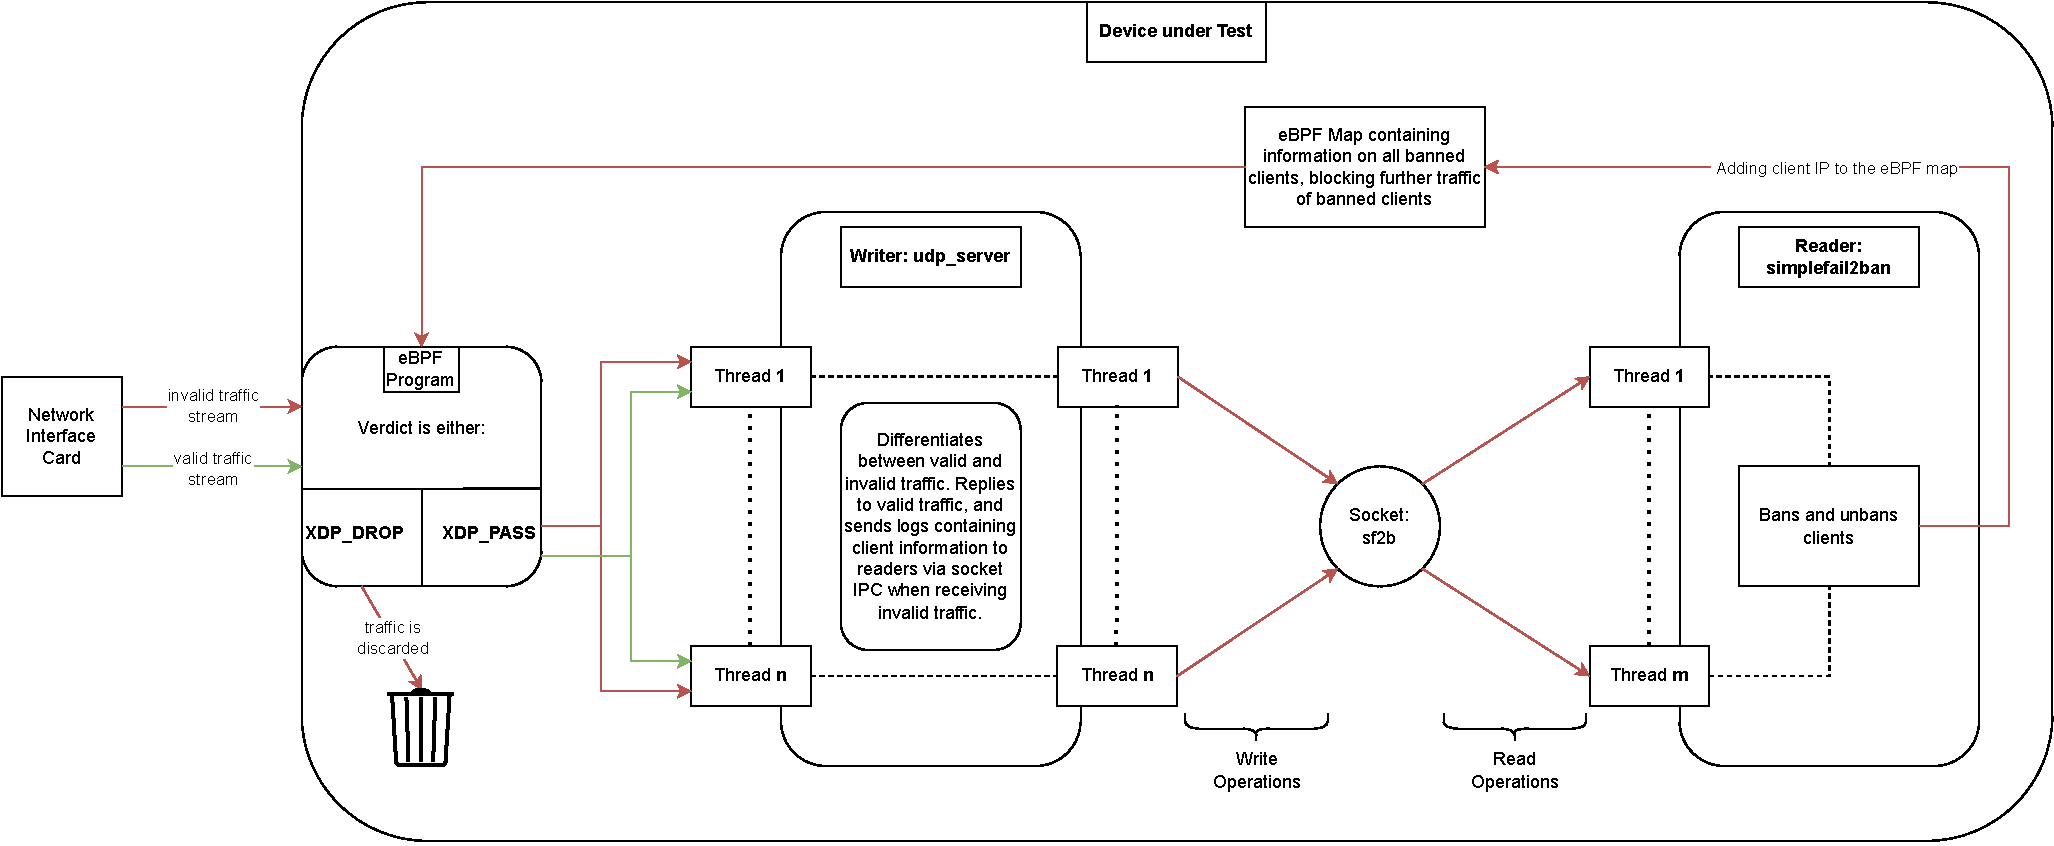
\includegraphics[width=1.\linewidth]{images/MeasurementArchitecture.pdf}
    \end{center}
\end{frame}

\begin{frame}{Factors and their levels}
    \begin{enumerate}
        \item IP stack: IPv4, IPv6 and IPv4/IPv6 mixed
        \item Effects of differing amount of invalid traffic sent: 100k, 1M, 10M, 20M, 30M PPS
        \item Effects of differing number of clients sending invalid data: 65,534 (from 256 subnets) and 131,068 (from 512 subnets)
        \item Differing IPC type\@: FILE (traditional file-based logging), SHM (using shared memeory), SOCK (using UNIX domain sockets)
            \begin{itemize}
                \item If applicable\@: No 2nd Reader/ Enabling 2nd Reader
            \end{itemize}
    \end{enumerate}
\end{frame}

\subsection{Evaluation of measurement data}
\begin{frame}{File pass: IPv4 - 65534 Clients - 30M invalid PPS}
    \begin{center}
        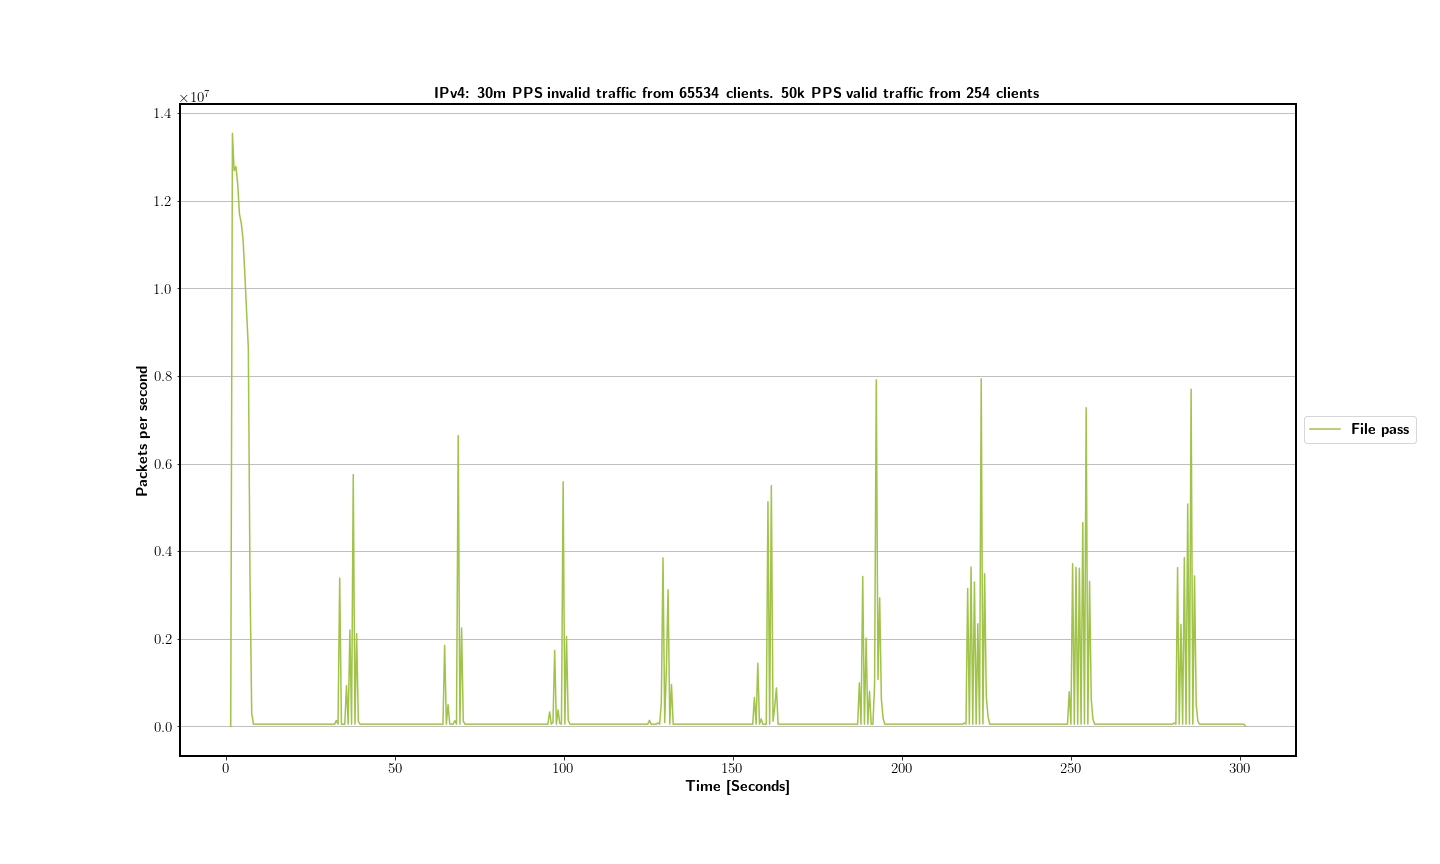
\includegraphics[width=1.\linewidth]{images/IPv4_30m_65534_1_file_pass.png}
    \end{center}
\end{frame}

\begin{frame}{Shm pass: IPv4 - 65534 Clients - 30M invalid PPS}
    \begin{center}
        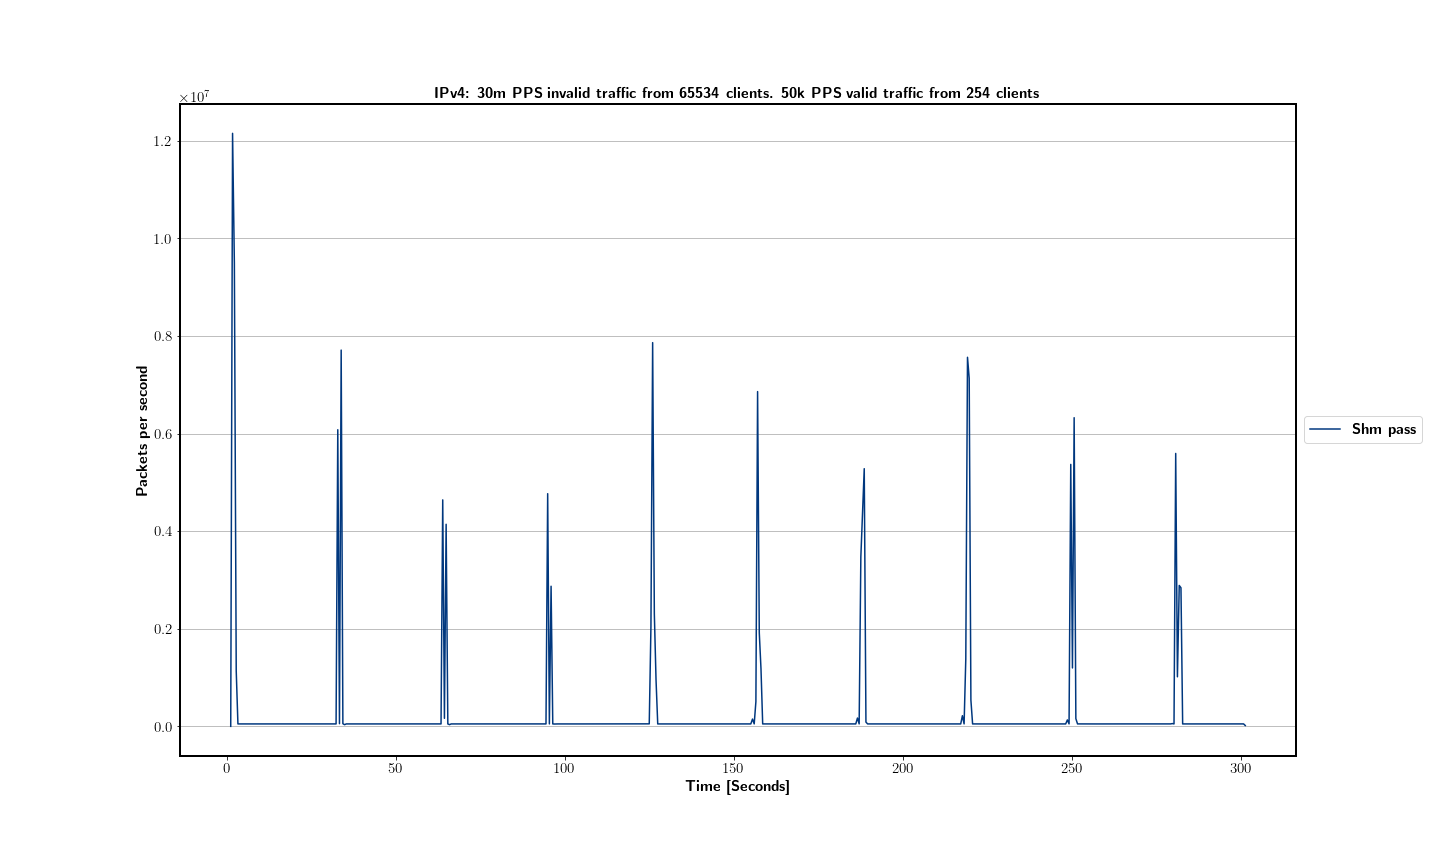
\includegraphics[width=1.\linewidth]{images/IPv4_30m_65534_1_shm_pass.png}
    \end{center}
\end{frame}

\begin{frame}{Sock pass: IPv4 - 65534 Clients - 30M invalid PPS}
    \begin{center}
        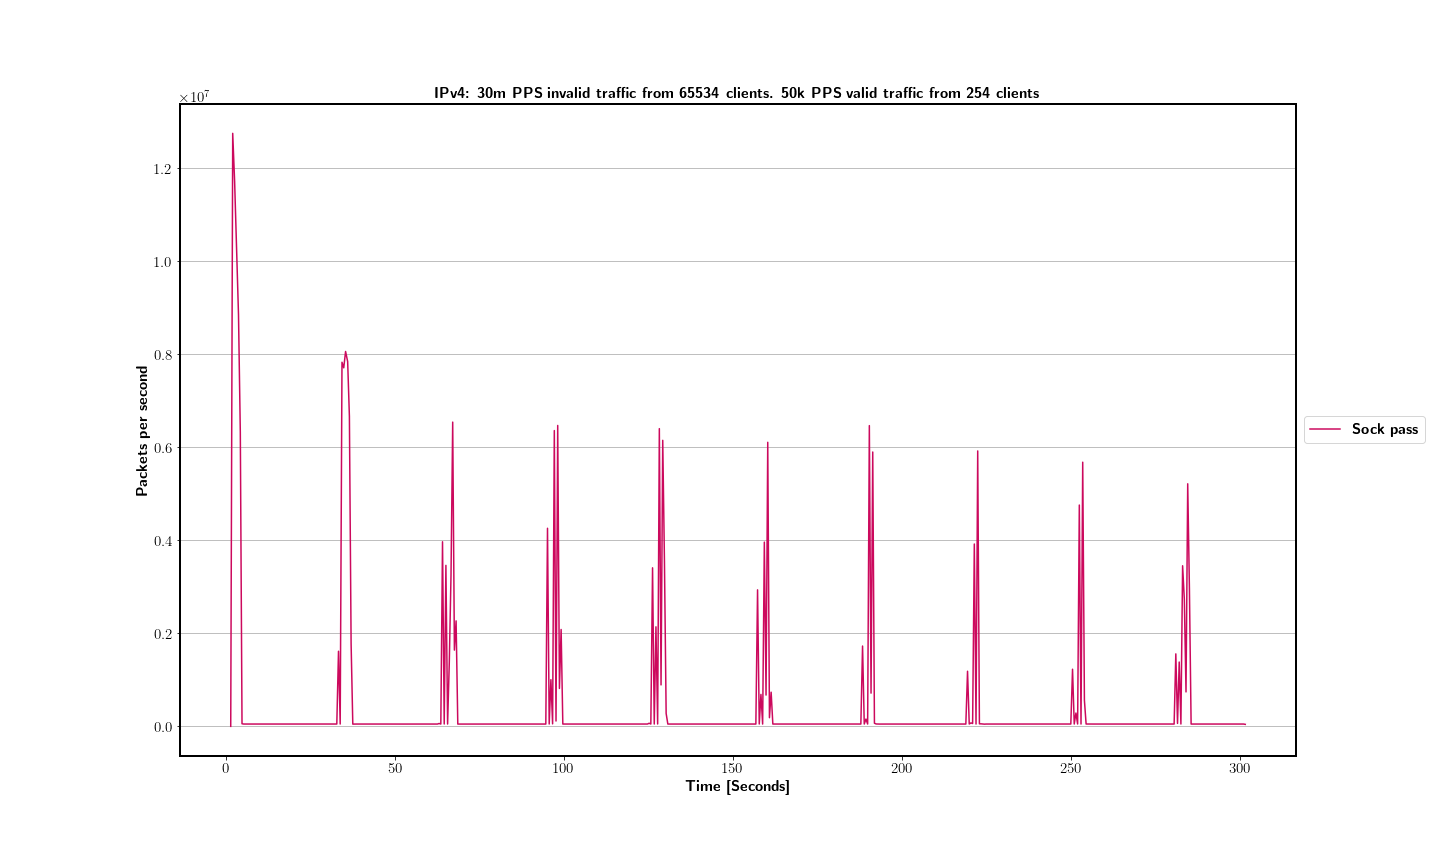
\includegraphics[width=1.\linewidth]{images/IPv4_30m_65534_1_sock_pass.png}
    \end{center}
\end{frame}

\begin{frame}{File drop: IPv4 - 65534 Clients - 30M invalid PPS}
    \begin{center}
        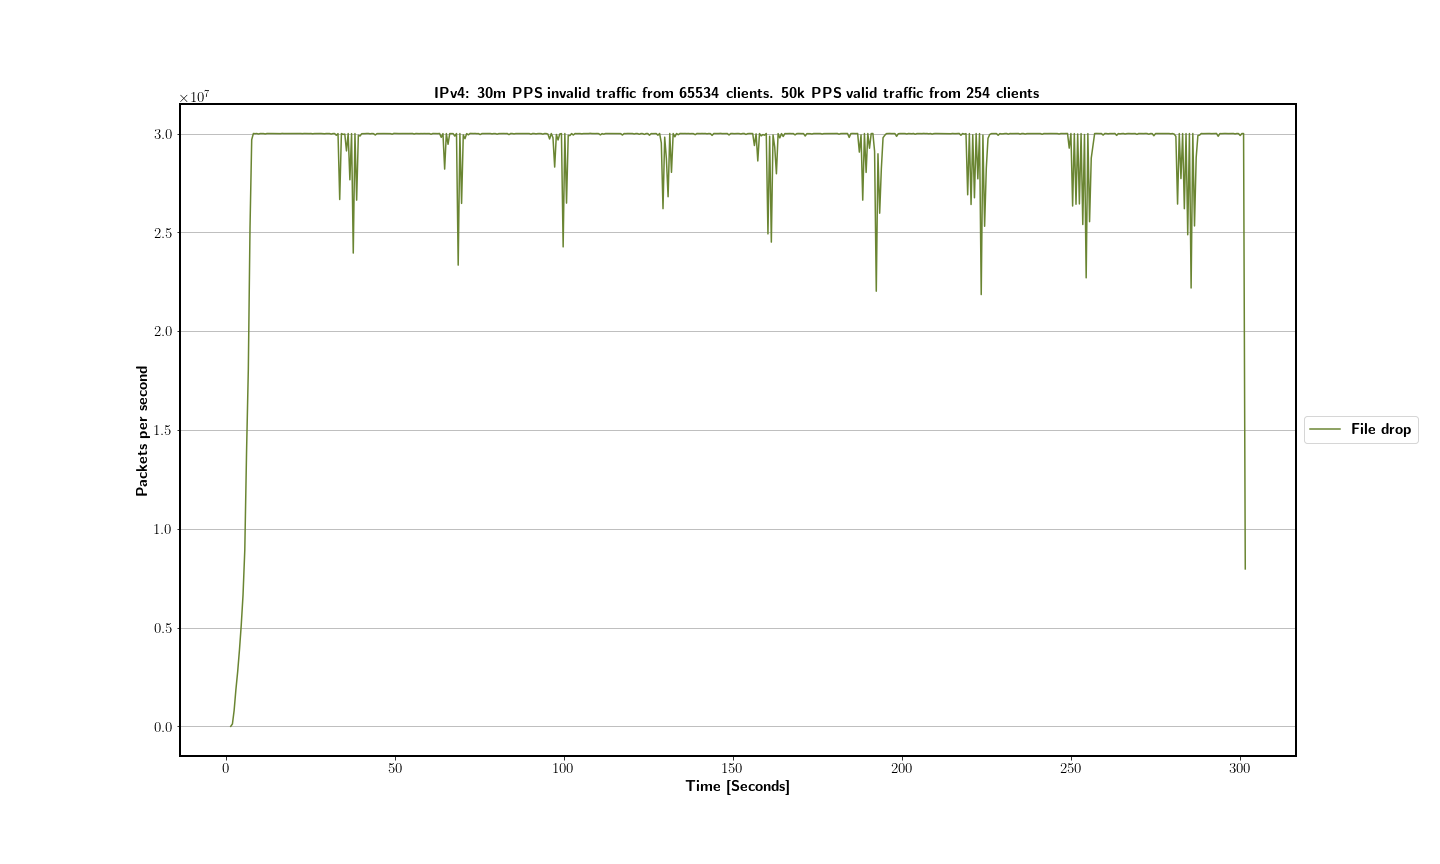
\includegraphics[width=1.\linewidth]{images/IPv4_30m_65534_1_file_drop.png}
    \end{center}
\end{frame}

\begin{frame}{Shm drop: IPv4 - 65534 Clients - 30M invalid PPS}
    \begin{center}
        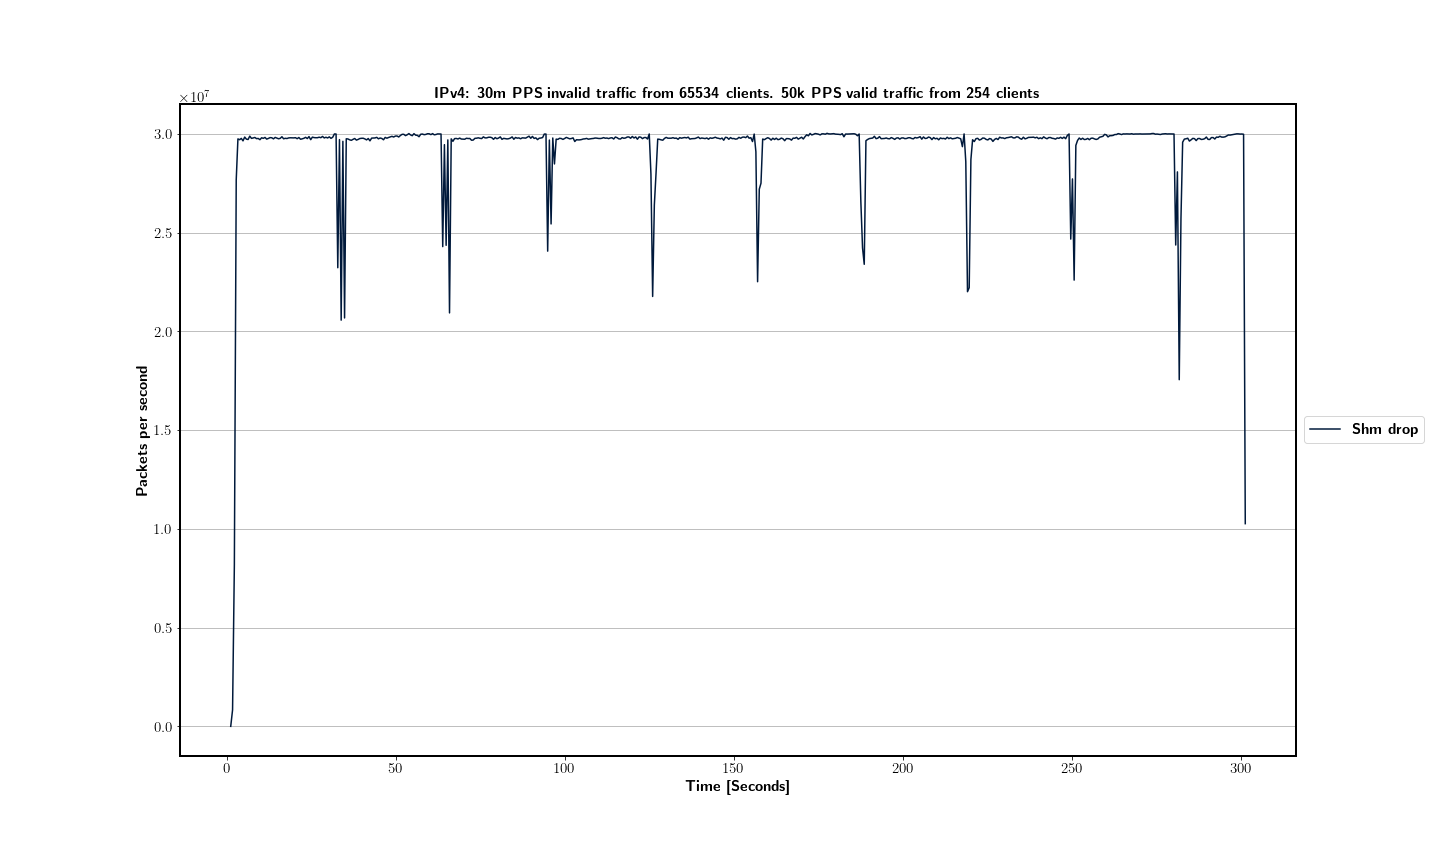
\includegraphics[width=1.\linewidth]{images/IPv4_30m_65534_1_shm_drop.png}
    \end{center}
\end{frame}

\begin{frame}{Sock drop: IPv4 - 65534 Clients - 30M invalid PPS}
    \begin{center}
        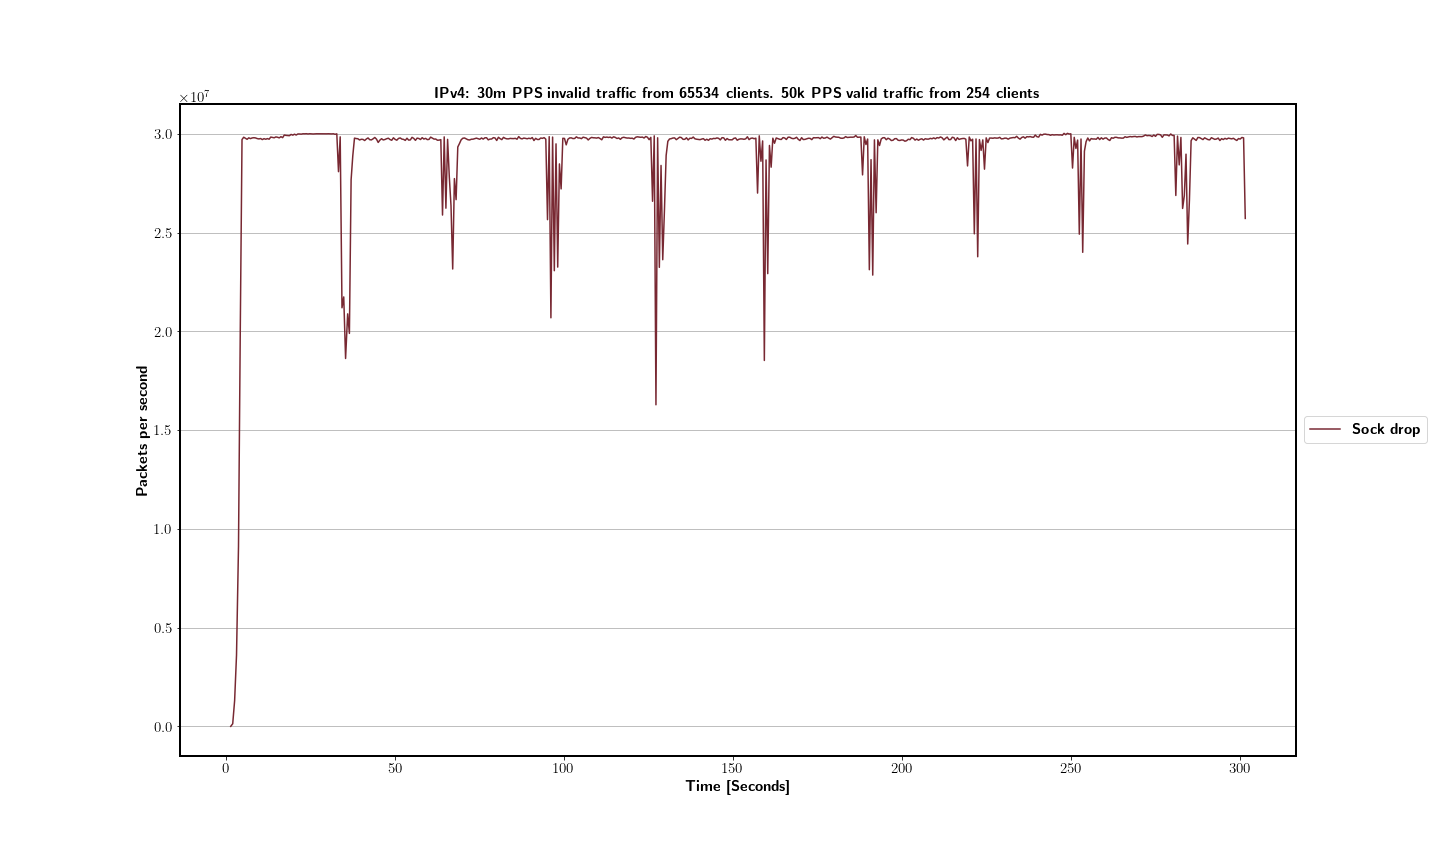
\includegraphics[width=1.\linewidth]{images/IPv4_30m_65534_1_sock_drop.png}
    \end{center}
\end{frame}

\begin{frame}{IPv4 - 65534 Clients - 30M invalid PPS - 50k valid PPS}
    \begin{center}
        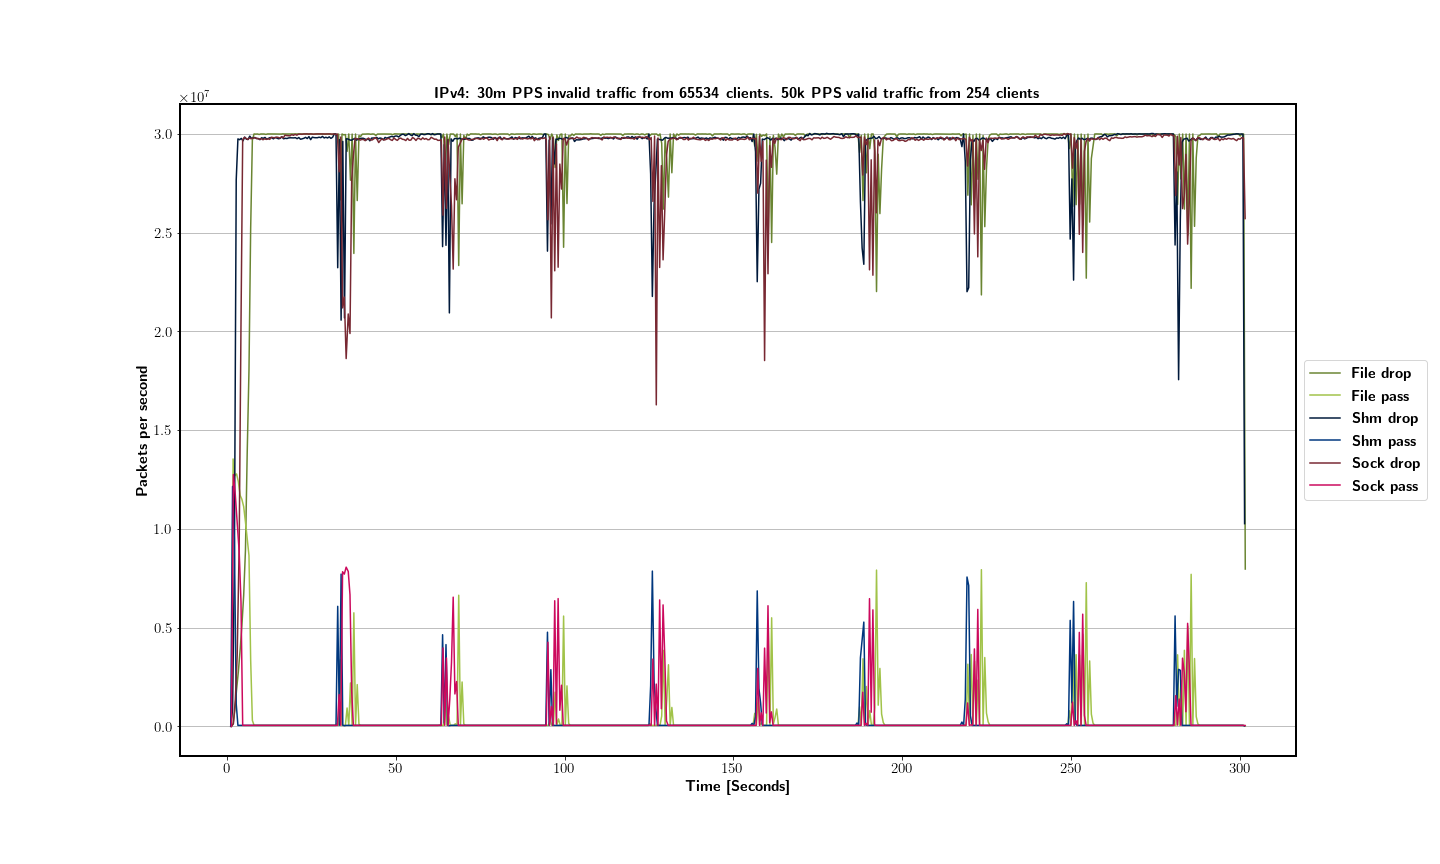
\includegraphics[width=1.\linewidth]{images/IPv4_30m_65534_1.png}
    \end{center}
\end{frame}

\begin{frame}{IPv4 - 65534 Clients - 30M invalid PPS - 50k valid PPS}
    \resizebox{\linewidth}{!}{%
    \begin{tabular}{l|l|l|l}
		\textbf{IPC type} & \textbf{XDP\_DROP [$10^8$]} & \textbf{XDP\_PASS [$10^6$]} & \textbf{Relative drop [\%]}\\
        \hline
		File & 87.75 & 159.82 & 97.52375345 \\
        Shm & 88.30 & 87.23 & 98.13105047 \\
        Sock & 87.45 & 139.42 & 97.18179422 \\
	\end{tabular}}
    \phantom{Filler}\\
    \phantom{Filler}\\
    \phantom{Filler}\\
    \resizebox{\linewidth}{!}{%
    \begin{tabular}{l|l|l|l}
		\textbf{IPC type} & \textbf{Packets received by udp\_server [$10^6$]} & \textbf{Log messages [$10^6$]} & \textbf{CPU [seconds]}\\
        \hline
		File & 17.48 & 4.07 & 16.55 \\
        Shm & 21.39 & 6.99 & 39.08 \\
        Sock & 16.92 & 3.16 & 138.85 \\
	\end{tabular}}
    \phantom{Filler}\\
    \begin{block}{Block}
        Total packets sent: 9,015m. Best-case drop rate: 99.97815533\%
    \end{block}
\end{frame}

\begin{frame}{IPv6 - 65534 Clients - 30M invalid PPS - 50k valid PPS}
    \begin{center}
        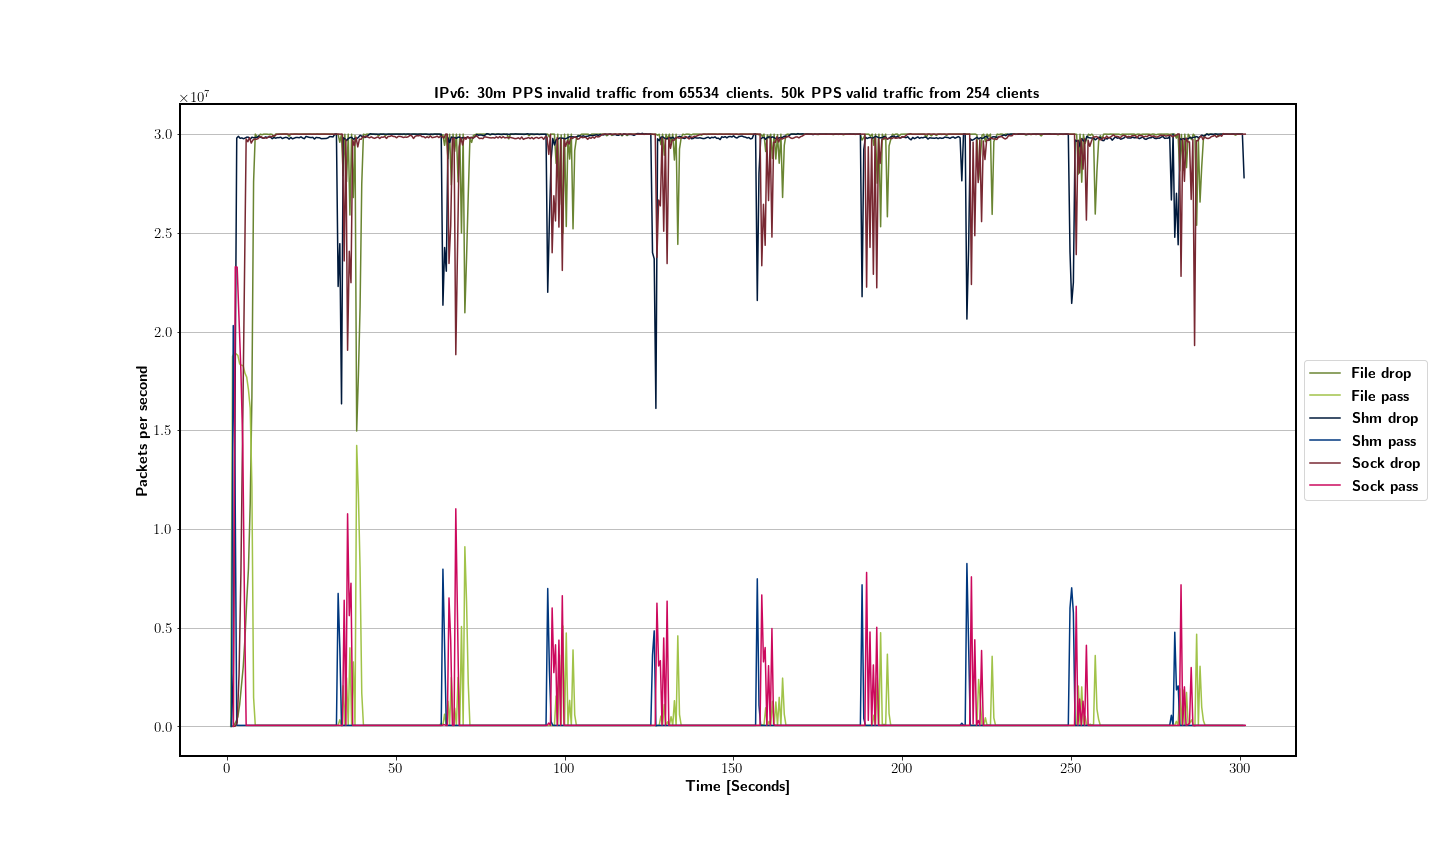
\includegraphics[width=1.\linewidth]{images/IPv6_30m_65534_1}
    \end{center}
\end{frame}

\begin{frame}{IPv6 - 65534 Clients - 30M invalid PPS - 50k valid PPS}
    \resizebox{\linewidth}{!}{%
    \begin{tabular}{l|l|l|l}
		\textbf{IPC type} & \textbf{XDP\_DROP [$10^8$]} & \textbf{XDP\_PASS [$10^6$]} & \textbf{Relative drop [\%]} \\
        \hline
		File & 87.41 & 211.05 & 97.14091697 \\
        Shm & 88.63 & 85.55 & 98.50239609 \\
        Sock & 87.77 & 170.03 & 97.54838057 \\
	\end{tabular}}
    \phantom{Filler}\\
    \phantom{Filler}\\
    \phantom{Filler}\\
    \resizebox{\linewidth}{!}{%
    \begin{tabular}{l|l|l|l}
		\textbf{IPC type} & \textbf{Packets received by udp\_server [$10^6$]} & \textbf{Log messages [$10^6$]} & \textbf{CPU [seconds]} \\
        \hline
		File & 17.20 & 3.87 & 22.51 \\
        Shm & 21.79 & 7.24 & 46.03 \\
        Sock & 16.92 & 3.00 & 149.69 \\
	\end{tabular}}
    \phantom{Filler}\\
    \begin{block}{Block}
        Total packets sent: 9,015m. Best-case drop rate: 99.97815533\%
    \end{block}
\end{frame}


\begin{frame}{IPv4 - 131068 Clients - 100k invalid PPS - 50k valid PPS}
    \begin{center}
        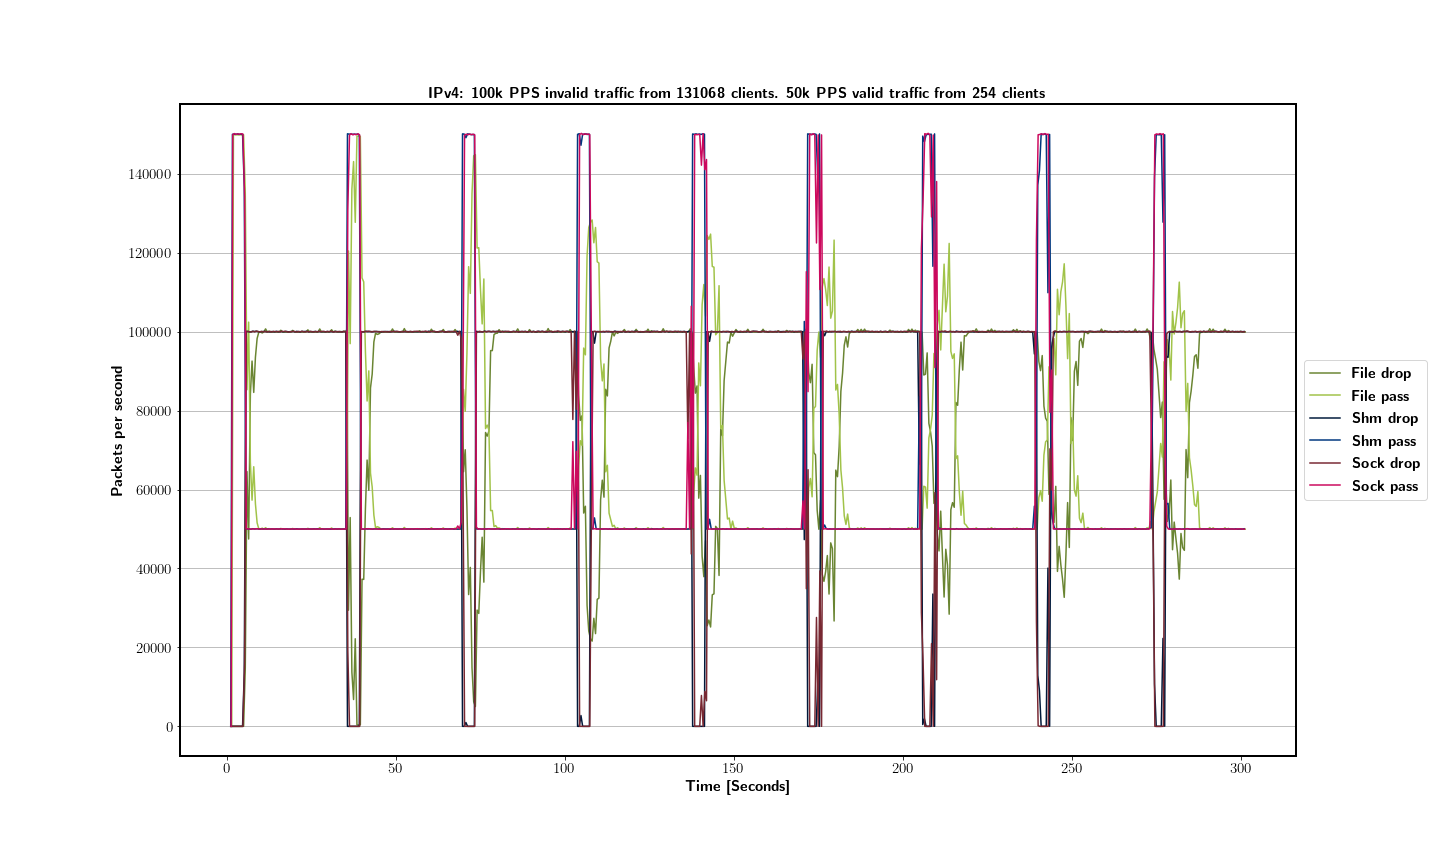
\includegraphics[width=1.\linewidth]{images/IPv4_100k_131068_1.png}
    \end{center}
\end{frame}

\begin{frame}{IPv4 - 131068 Clients - 100k invalid PPS - 50k valid PPS}
    \resizebox{\linewidth}{!}{%
    \begin{tabular}{l|l|l|l}
		\textbf{IPC type} & \textbf{XDP\_DROP [$10^6$]} & \textbf{XDP\_PASS [$10^6$]} & \textbf{Relative drop [\%]} \\
        \hline
		File & 25.99 & 19.01 & 99.69409958 \\
        Shm & 26.46 & 18.54 & 101.5083842 \\
        Sock & 26.44 & 18.56 & 101.4395334 \\
	\end{tabular}}
    \phantom{Filler}\\
    \phantom{Filler}\\
    \phantom{Filler}\\
    \resizebox{\linewidth}{!}{%
    \begin{tabular}{l|l|l|l}
		\textbf{IPC type} & \textbf{Packets received by udp\_server [$10^6$]} & \textbf{Log messages [$10^6$]} & \textbf{CPU [seconds]} \\
        \hline
		File & 18.16 & 3.54 & 08.34 \\
        Shm & 18.54 & 3.54 & 10.14 \\
        Sock & 18.53 & 3.54 & 100.40 \\
	\end{tabular}}
    \phantom{Filler}\\
    \begin{block}{Block}
        Total packets sent: 45m. Best-case drop rate: 86.8932\%
    \end{block}
\end{frame}

\begin{frame}{IPv4 - 131068 Clients - 30M invalid PPS - 50k valid PPS}
    \begin{center}
        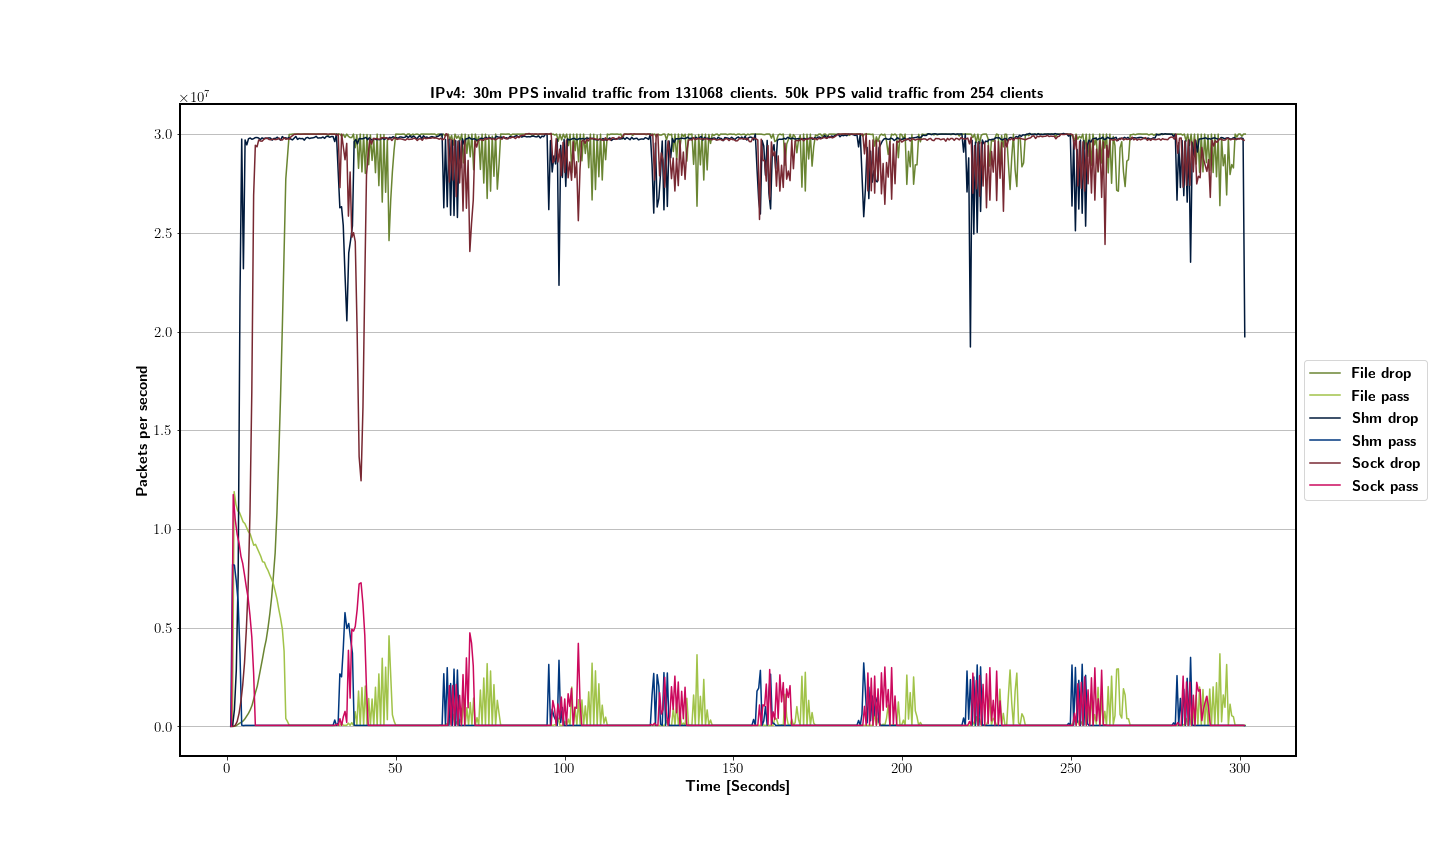
\includegraphics[width=1.\linewidth]{images/IPv4_30m_131068_2.png}
    \end{center}
\end{frame}

\begin{frame}{IPv4 - 131068 Clients - 30M invalid PPS - 50k valid PPS}
    \resizebox{\linewidth}{!}{%
    \begin{tabular}{l|l|l|l}
        \textbf{IPC type} & \textbf{XDP\_DROP [$10^8$]} & \textbf{XDP\_PASS [$10^6$]} & \textbf{Relative drop [\%]} \\
        \hline
		File & 85.02 & 238.30 & 94.51036756 \\
        Shm & 87.57 & 104.14 & 97.33826458 \\
        Sock & 86.12 & 180.89 & 95.73084169 \\
	\end{tabular}}
    \phantom{Filler}\\
    \phantom{Filler}\\
    \phantom{Filler}\\
    \resizebox{\linewidth}{!}{%
    \begin{tabular}{l|l|l|l}
        \textbf{IPC type} & \textbf{Packets received by udp\_server [$10^6$]} & \textbf{Log messages [$10^6$]} & \textbf{CPU [seconds]} \\
        \hline
		File & 18.04 & 7.44 & 38.99 \\
        Shm & 25.32 & 11.50 & 71.92 \\
        Sock & 18.33 & 5.93 & 323.02 \\
	\end{tabular}}
    \phantom{Filler}\\
    \begin{block}{Block}
        Total packets sent: 9,015m. Best-case drop rate: 99.95631067\%
    \end{block}
\end{frame}

\begin{frame}{IPv6 - 131068 Clients - 30M invalid PPS - 50k valid PPS}
    \begin{center}
        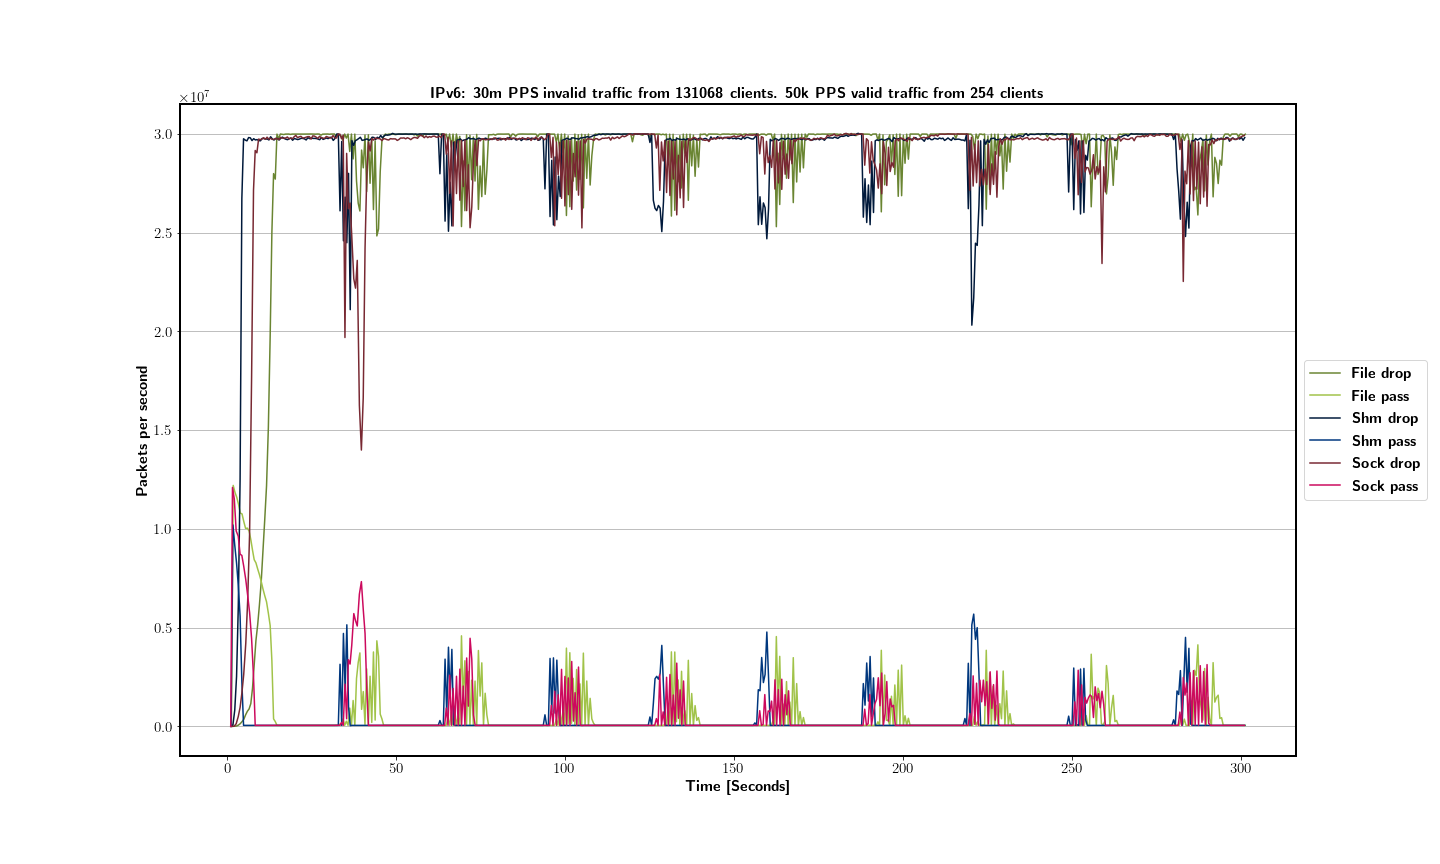
\includegraphics[width=1.\linewidth]{images/IPv6_30m_131068_1.png}
    \end{center}
\end{frame}

\begin{frame}{IPv6 - 131068 Clients - 30M invalid PPS - 50k valid PPS}
    \resizebox{\linewidth}{!}{%
    \begin{tabular}{l|l|l|l}
        \textbf{IPC type} & \textbf{XDP\_DROP [$10^8$]} & \textbf{XDP\_PASS [$10^6$]} & \textbf{Relative drop [\%]} \\
        \hline
		File & 85.73 & 228.07 & 95.29278185 \\
        Shm & 87.60 & 109.08 & 97.37706621 \\
        Sock & 86.21 & 177.33 & 95.82614459 \\
	\end{tabular}}
    \phantom{Filler}\\
    \phantom{Filler}\\
    \phantom{Filler}\\
    \resizebox{\linewidth}{!}{%
    \begin{tabular}{l|l|l|l}
        \textbf{IPC type} & \textbf{Packets received by udp\_server [$10^6$]} & \textbf{Log messages [$10^6$]} & \textbf{CPU [seconds]} \\
        \hline
		File & 17.90 & 6.91 & 38.41 \\
        Shm & 25.08 & 11.15 & 74.71 \\
        Sock & 18.67 & 6.18 & 317.37 \\
	\end{tabular}}
    \phantom{Filler}\\
    \begin{block}{Block}
        Total packets sent: 9,015m. Best-case drop rate: 99.95631067\%
    \end{block}
\end{frame}

\begin{frame}{IPv4v6 - 131068 Clients - 30M invalid PPS - 50k valid PPS}
    \begin{center}
        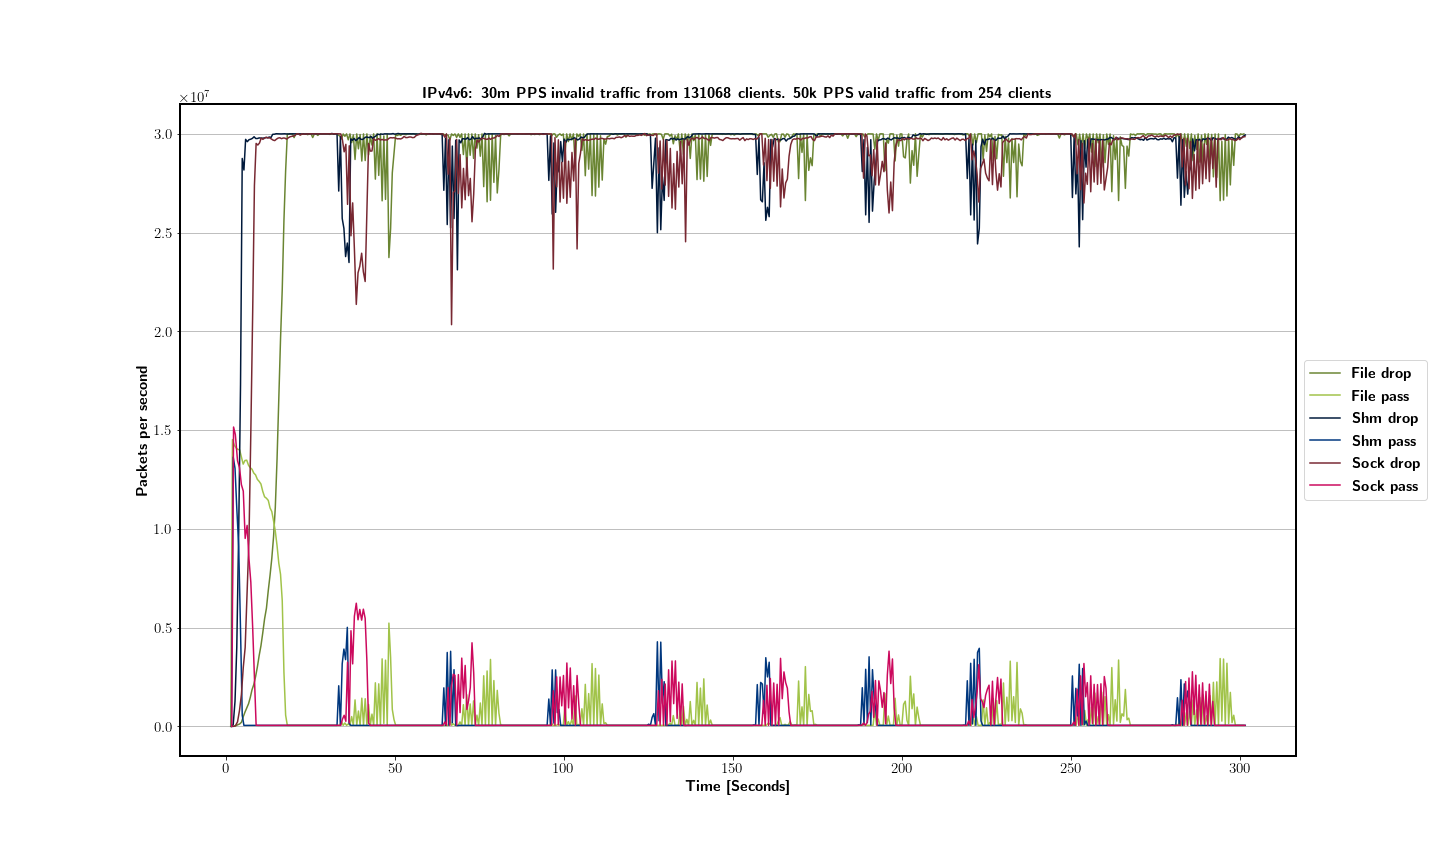
\includegraphics[width=1.\linewidth]{images/IPv4v6_30m_131068_2.png}
    \end{center}
\end{frame}

\begin{frame}{IPv4v6 - 131068 Clients - 30M invalid PPS - 50k valid PPS}
    \resizebox{\linewidth}{!}{%
    \begin{tabular}{l|l|l|l}
        \textbf{IPC type} & \textbf{XDP\_DROP [$10^8$]} & \textbf{XDP\_PASS [$10^6$]} & \textbf{Relative drop [\%]} \\
        \hline
		File & 85.12 & 286.15 & 94.61335186 \\
        Shm & 88.02 & 105.83 & 97.84149307 \\
        Sock & 86.30 & 212.81 & 95.93428297 \\
	\end{tabular}}
    \phantom{Filler}\\
    \phantom{Filler}\\
    \phantom{Filler}\\
    \resizebox{\linewidth}{!}{%
    \begin{tabular}{l|l|l|l}
        \textbf{IPC type} & \textbf{Packets received by udp\_server [$10^6$]} & \textbf{Log messages [$10^6$]} & \textbf{CPU [seconds]} \\
        \hline
		File & 17.69 & 7.07 & 47.15 \\
        Shm & 25.13 & 11.16 & 94.64 \\
        Sock & 18.00 & 5.99 & 353.34 \\
	\end{tabular}}
    \phantom{Filler}\\
    \begin{block}{Block}
        Total packets sent: 9,015m. Best-case drop rate: 99.95631067\%
    \end{block}
\end{frame}

\begin{frame}{IPv4v6 2nd Reader - 131068 Clients - 1M invalid PPS - 50k valid PPS}
    \begin{center}
        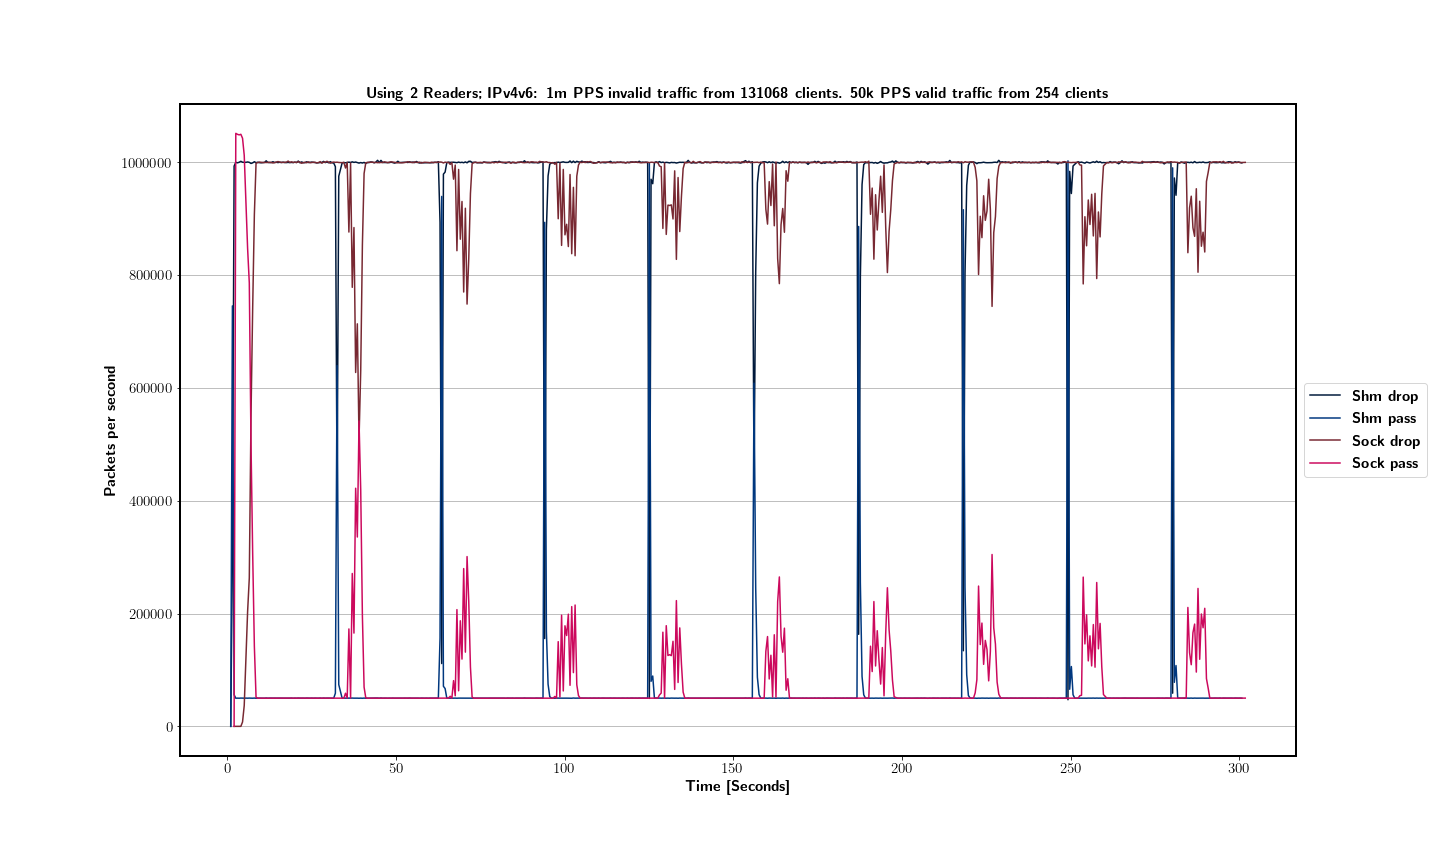
\includegraphics[width=1.\linewidth]{images/IPv4v6_1m_2ndReader_1.png}
    \end{center}
\end{frame}

\begin{frame}{IPv4v6 2nd Reader - 131068 Clients - 1M invalid PPS - 50k valid PPS}
    \resizebox{\linewidth}{!}{%
    \begin{tabular}{l|l|l|l}
        \textbf{IPC type} & \textbf{XDP\_DROP [$10^7$]} & \textbf{XDP\_PASS [$10^6$]} & \textbf{Relative drop [\%]} \\
        \hline
		Shm & 29.53 & 19.75 & 99.72283593 \\
        Sock & 28.91 & 25.94 & 97.6334018 \\
	\end{tabular}}
    \phantom{Filler}\\
    \phantom{Filler}\\
    \phantom{Filler}\\
    \resizebox{\linewidth}{!}{%
    \begin{tabular}{l|l|l|l}
        \textbf{IPC type} & \textbf{Packets received by udp\_server [$10^6$]} & \textbf{Log messages [$10^6$]} & \textbf{CPU [seconds]} \\
        \hline
		Shm & 19.48 & 4.49 & 17.76 \\
        Sock & 18.29 & 4.15 & 80.82 \\
	\end{tabular}}
    \phantom{Filler}\\
    \begin{block}{Block}
        Total packets sent: 9,015m. Best-case drop rate: 99.95631067\%
    \end{block}
\end{frame}

\begin{frame}{IPv4v6 2nd Reader - 131068 Clients - 20M invalid PPS - 50k valid PPS}
    \begin{center}
        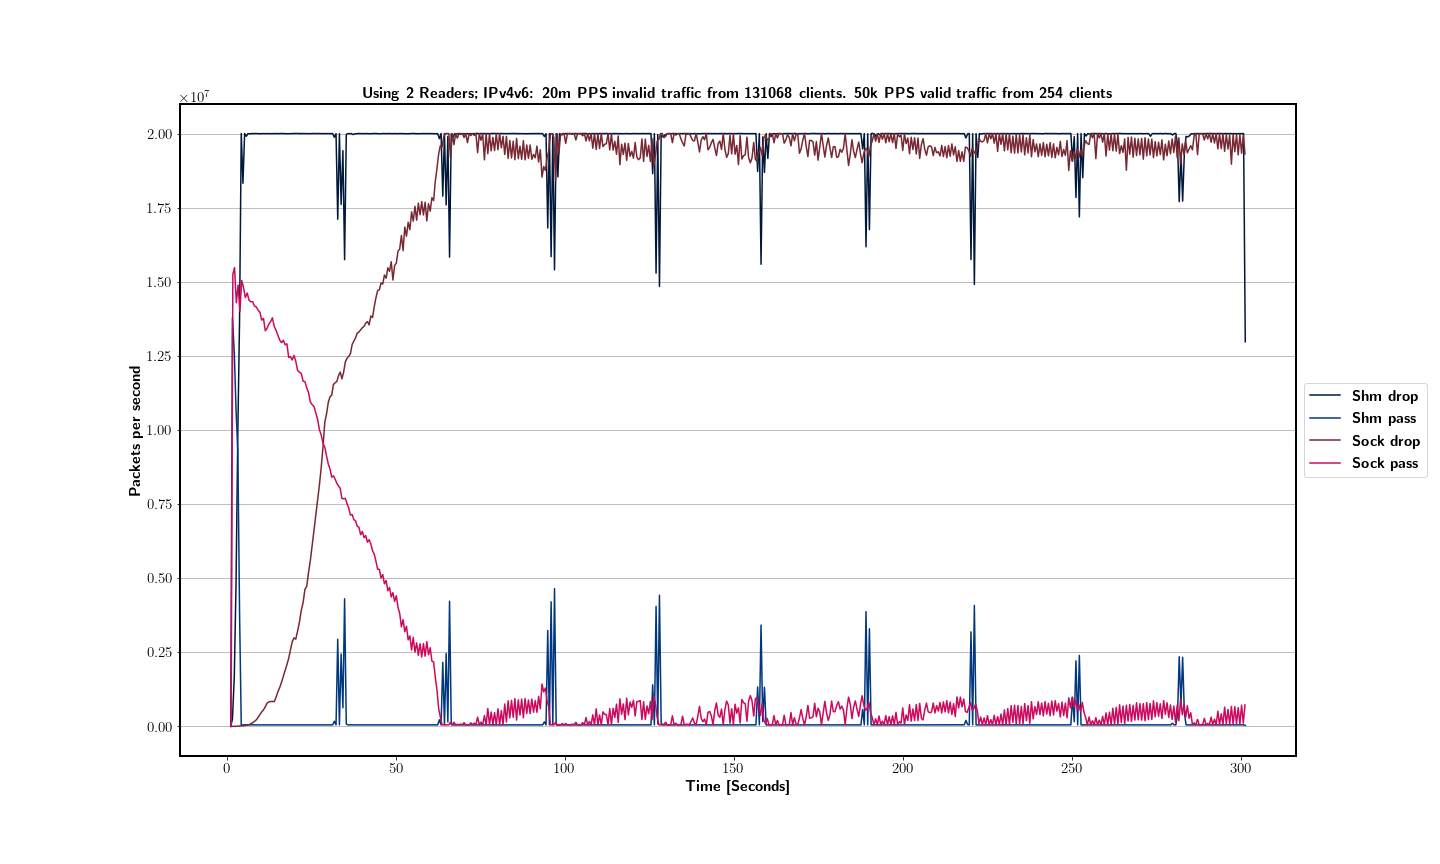
\includegraphics[width=1.\linewidth]{images/IPv4v6_20m_2ndReader_1.png}
    \end{center}
\end{frame}

\begin{frame}{IPv4v6 2nd Reader - 131068 Clients - 30M invalid PPS - 50k valid PPS}
    \begin{center}
        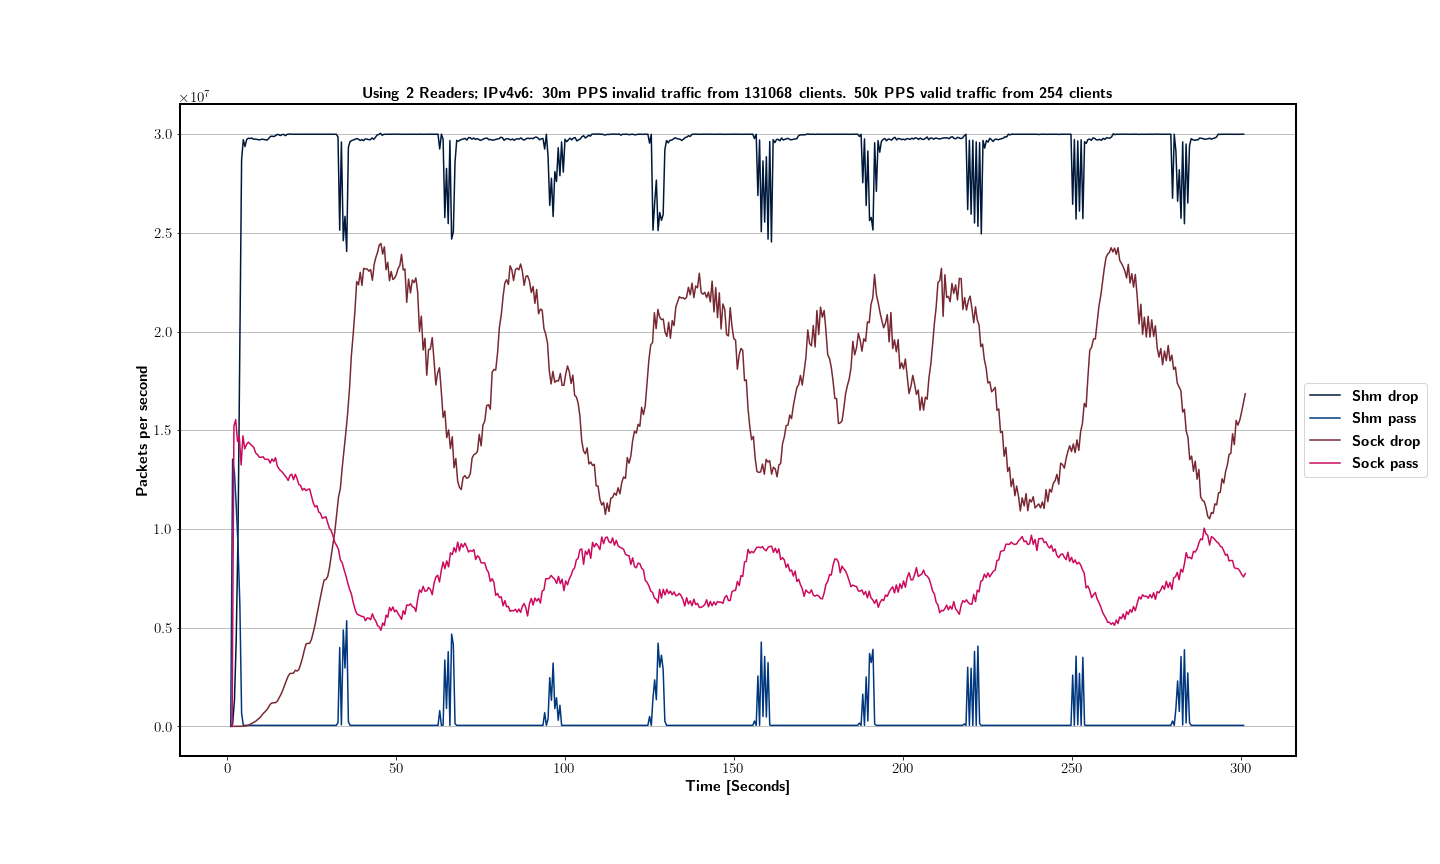
\includegraphics[width=1.\linewidth]{images/IPv4v6_30m_2ndReader_1.png}
    \end{center}
\end{frame}

\begin{frame}{Questions?}
    Questions?
\end{frame}

\cleardoublepage
\backupbegin
\pagenumbering{arabic}

\backupend
\end{document}
